\documentclass[english,12pt,twoside,a4paper]{report}
    \usepackage[ngerman,english]{babel,varioref}		% language
    \usepackage[ddmmyyyy]{datetime}
    \usepackage[utf8]{inputenc}
    \usepackage[T1]{fontenc}
    \usepackage{pslatex}
    \usepackage{amsmath}
    \usepackage{multirow}
    \usepackage{microtype}
    \usepackage{ellipsis}
    \usepackage{textcomp}
    \usepackage{longtable}
    \usepackage{rotating}
    \usepackage[section]{placeins}

    \usepackage{caption}		% Customize caption aesthetics
    \usepackage{subcaption}

	\usepackage{graphicx}		% required to insert images
    \usepackage[space]{grffile} % insert images baring a filename which contains spaces
	\usepackage{float}			% allow to forcefully set the location of an object

    %\usepackage[osf,sc]{mathpazo}  % Palatino als Schriftart
    %\usepackage{charter}
    \newcommand{\U}[1]{\underline{#1}}
    \newcommand{\grad}{\text{grad }}
    \newcommand{\dive}{\text{div }}
    \newcommand{\rot}{\text{rot }}
    \newcommand{\B}[1]{\textbf{#1}}
    \makeatletter
    \makeatother

    %\usepackage{geometry,mflogo,xspace,texnames,path,booktabs,bm}

    \usepackage[bookmarks]{hyperref}
    \usepackage{thumbpdf}

    \pagestyle{headings}                 % Seitenstil
    \oddsidemargin0.8cm                  % linker Rand fuer ungerade Seiten bei \twoside
    \evensidemargin0.2cm                 % linker Rand fuer gerade Seiten (nur bei \twoside)
    \topmargin0.5cm                      % oberer Rand bis zur Oberseite Kopfzeile
    \textheight21cm                      % Texth"ohe auf einer Seite
    \textwidth15cm                       % Textbreite auf einer Seite
    \renewcommand{\topfraction}{0.75}    % Anteil der Gleitk"asten am Seitenanfang
    \renewcommand{\bottomfraction}{0.75} % Anteil der Gleitk"asten am Seitenende
    \parskip1ex  plus1ex minus0.5ex      % Abstand zwischen Abs"atzen
    \parindent0em                        % Einr"uckung der ersten Zeile eines Absatzes
    \newcommand{\clearemptydoublepage}{\newpage{\pagestyle{empty}\cleardoublepage}}

    \title{Optimization of Particle Identification}
    \author{\href{mailto:gordian.edenhofer@gmail.com}{Gordian Edenhofer}}
    \date{29. June 2018}

\begin{document}

\selectlanguage{english}

\pagenumbering{Roman}
%\maketitle
\thispagestyle{empty}
\begin{center}
	\selectlanguage{ngerman}

	\begin{LARGE}
		{
		\bf
		\hspace*{1cm} Optimierung der Teilchenidentifizierung \\ [0.3cm]
		}
	\end{LARGE}
	\vspace{0.5cm}
	%
	\begin{figure}[htbp]
		\begin{center}
			\hspace*{1cm}
			
\includegraphics[height=4cm]{{{../res/LMU logo}}}
		\end{center}
		%\label{fig-lmulogo}
	\end{figure}

	\vspace{1.0cm}
	\begin{large}
		\hspace*{1cm}Bachelorarbeit an der Fakultät für Physik \\
		\hspace*{1cm}der \\
		\hspace*{1cm}Ludwig-Maximilians-Universität~München \\ [2.5cm]

		\hspace*{1cm}vorgelegt von \\
		{
		\bf
		\hspace*{1cm}Gordian~Edenhofer \\
		}
		\hspace*{1cm}geboren in Frankfurt am Main am \datengerman\formatdate{13}{07}{1997} \\ [0.5cm]

		\hspace*{1cm}München, den \datengerman\formatdate{29}{06}{2018} \\ [0.5cm]

		\hspace*{1cm}Betreuer: \\
		{
		\bf
		\hspace*{1cm}Prof.~Dr.~Thomas~Kuhr
		}
	\end{large}
\end{center}

\clearpage
\thispagestyle{empty}
\mbox{ }
\setcounter{page}{0}
\clearpage
\thispagestyle{empty}
\begin{center}
	\begin{LARGE}
		{
			\bf
			\hspace*{1cm} Optimization of Particle Identification \\ [0.3cm]
		}
	\end{LARGE}
	\vspace{0.5cm}
	%
	\begin{figure}[htbp]
		\begin{center}
			\hspace*{1cm}
			
\includegraphics[height=4cm]{pics/lmu3.pdf}
		\end{center}
		%\label{fig-lmulogo}
	\end{figure}

	\vspace{1.0cm}
	\begin{large}
		\hspace*{1cm}Bachelor thesis at the faculty of physics \\
		\hspace*{1cm}of the \\
		\hspace*{1cm}Ludwig-Maximilians-Universität München \\ [2.5cm]
		\hspace*{1cm}handed in by \\
		{\bf
		\hspace*{1cm}Gordian Edenhofer \\ }
		\hspace*{1cm}born in Frankfurt am Main on the \formatdate{13}{07}{1997} \\ [0.5cm]
		%\hspace*{1cm}\today
		\hspace*{1cm}Munich, the \formatdate{28}{06}{2018}
	\end{large}
\end{center}

\clearpage
\thispagestyle{empty}
\mbox{ }
\setcounter{page}{0}
%\clearpage
%\chapter*{Abstract}

This study aims at evaluating further particle identification approaches.
At first the goodness of the detector variables is measured. Flaws are outlined and possible causes are evaluated. Afterwards further techniques are discussed which combine the detector variables in a new way.

A Bayesian approach to particle identification is discussed. It aims at producing probabilities of a track belonging to a particle species in dependance of the received signal. The process of obtaining the conditional probabilities is described in greater detail. In addition, some extensions to the Bayesian approach are presented and evaluated. Flaws and benefits are compared using a generic decay.

Lastly, a neural network is used to label particle tracks. For a simple network, different methods to adapt the weights and various input forms are evaluated. Hereby, tools from machine learning and statistics are discussed and their application is outlined. In the end the accuracy of the network on a generic decay is determined.

\clearpage

\tableofcontents

\cleardoublepage

\pagenumbering{arabic}

\chapter{Statistics for particle analysis}
\label{chap:statistics}

\section{Classification functions}
\label{sec:classification_functions}

A main part of identifying particles is to examine statistical measures. The main concepts used throughout the thesis heavily relies on such values to compare the goodness of a identification method. However their use is not limited to physics, let alone particle physics, but spans over all field containing some form of (binary) classification problems.
In the following explanatory paragraphs it is assumed that one wants to identify kaons in a set of data containing a multitude of alternative particles.

The most important classification functions are:
\begin{itemize}
	\item \textbf{T}rue \textbf{P}ositive \textbf{R}ate (\textbf{TPR}): \textit{Proportion of accepted elements which are correct relative to all positives}

	\nobreak
	Hence the ratio of identified kaons which actually were kaons in proportion to the number of kaons in the data.

	\item \textbf{T}rue \textbf{N}egative \textbf{R}ate or Specificity (\textbf{TNR}): \textit{Proportion of rejected elements which are incorrect relative to all negatives}

	\nobreak
	In our example this would translate to the ratio of non-kaon particles being identified as non-kaons in proportion to the number of all non-kaon particles.

	\item \textbf{F}alse \textbf{P}ositive \textbf{R}ate (\textbf{FPR}): \textit{Proportion of accepted elements which are incorrect relative to all negatives}

	\nobreak
	This would translate to the fraction of non-kaon particles identified as kaons over the number of all non-kaons.

	\item \textbf{F}alse \textbf{N}egative \textbf{R}ate (\textbf{FNR}): \textit{Proportion of rejected elements which are correct relative to all positives}

	\nobreak
	Using our kaon sample once more; this would represent the fraction of kaons classified as being non-kaons over the number of all non-kaons.

	\item \textbf{P}ositive \textbf{P}redicted \textbf{V}alue (\textbf{PPV}): \textit{Proportion of accepted elements which are correct relative to all accepted}

	\nobreak
	Using our kaon sample one last time; this would represent the fraction of kaons classified as being as kaons over the number of all tracks classified as kaons but not necessarily being one.

\end{itemize}

In abstract terms; the two prefixes used above may be summarized as seen in \autoref{tab:classification_guidelines}. Bear in mind that `negative' and `positive' if used separately denote the presence of the desired feature and therefore does not fit the definition given in the table in this case.

\begin{table}[ht]
	\centering
	\begin{tabular}{l|ll}
		Veracity & True = correct & False = incorrect \\
		Identification & Positive = accepted & Negative = rejected
	\end{tabular}
	\caption{Guidelines for understanding the meaning of a classification function.}
	\label{tab:classification_guidelines}
\end{table}

\section{Receiver operating characteristic}
\label{sec:roc}

The \textbf{R}eceiver \textbf{O}perating \textbf{C}haracteristic (\textbf{ROC}) curve is the TPR plotted over the FPR. As such the values on the $x$ and $y$ axis go from $0$ to $1$. Each point on the curve represent an applied selection criterion on the data.

On a set of data with two equally likely yields a straight diagonal line connecting the point $(0, 0)$ with $(1, 1)$ would represent plain guessing. A curve below that would be worse and anything above, is some degree of good. An optimal curve would achieve a high TPR value at a very low FPR.
Multiple methods can therefore be compared by assessing how steep each methods TPR is rising relative to the FPR. The \autoref{fig:sample_roc_curve} visually underlines the above described relations.

\begin{figure}[ht]
	\centering
	\includegraphics[width=\textwidth,height=0.4\textheight,keepaspectratio]{{{../res/Sample Receiver Operating Characteristic (ROC) curve}}}
	\caption{Sample ROC curve for a binary classification problem with each outcome being equally likely.}
	\label{fig:sample_roc_curve}
\end{figure}

\section{Identification efficiencies}
\label{sec:efficiency}

In particle physics the identification efficiency is defined as the proportion of correctly classified particles relative to all the available particles belonging to that class. Hence it directly represents the PPV. Both terms will be used as synonyms throughout the thesis.

For an exclusive particle classification the $\epsilon_{PID}$-matrix is the confusion matrix normed by row. Each cell in a row represents the probability of a particle of that row's class being identified as the particle of that column's class. On the diagonal of that matrix it contains the identification efficiencies for a particle species.
The definition generalizes to non normed matrices, e.g. resulting from non-exclusive. Although reading the matrix is less intuitive as a particle might belong to multiple classes and makes comparing them very ambitious.

The values of the matrix are given by the fraction of particles $i$ classified as $j$ over the true abundance of particle $i$. As formula its values are

\begin{equation}
	\epsilon_{i j} = \frac{N_{i \text{ classified as } j}}{A_{i \text{ true}}}.
\end{equation}

For our six particle species with ID the matrix has the following shape:

\begin{equation}
	\begin{pmatrix}
		\epsilon_{K K} & \epsilon_{K \pi} & \epsilon_{K e} & \epsilon_{K \mu} & \epsilon_{K p} & \epsilon_{K d} \\
		\epsilon_{\pi K} & \epsilon_{\pi \pi} & \epsilon_{\pi e} & \epsilon_{\pi \mu} & \epsilon_{\pi p} & \epsilon_{\pi d} \\
		\epsilon_{e K} & \epsilon_{e \pi} & \epsilon_{e e} & \epsilon_{e \mu} & \epsilon_{e p} & \epsilon_{e d} \\
		\epsilon_{\mu K} & \epsilon_{\mu \pi} & \epsilon_{K e} & \epsilon_{K \mu} & \epsilon_{K p} & \epsilon_{\mu d} \\
		\epsilon_{p K} & \epsilon_{p \pi} & \epsilon_{p e} & \epsilon_{p \mu} & \epsilon_{p p} & \epsilon_{p d} \\
		\epsilon_{d K} & \epsilon_{d \pi} & \epsilon_{K e} & \epsilon_{K \mu} & \epsilon_{K p} & \epsilon_{d d} \\
	\end{pmatrix}.
\end{equation}

\section{Likelihood}
\label{sec:likelihood}

\subsection{Likelihood ratio}
\label{subsec:likelihood_ratios}

The ratio of likelihoods is commonly used for comparisons of the goodness of two models. Consider two alternative models, one parameterised by the hypothesis $H_0$, the other by $H_1$. Each yield a likelihood of event $\pmb{x}$ occurring given their hypothesis is true. Their ratio
\begin{equation*}
	\frac{\mathcal{L}(\pmb{x}|H_0)}{\mathcal{L}(\pmb{x}|H_1)}
\end{equation*} denotes how many times more likely the event $\pmb{x}$ is under hypothesis $H_0$ relative to $H_1$.

However the event $\pmb{x}$ must not necessarily take the form a simple one dimensional value. It may very well be a composition of e.g. in our case multiple detectors responses. Nevertheless if one assumes all constituents $x_i$ of $\pmb{x}$ are independent of each other, one may simple construct $\mathcal{L}(\pmb{x}|H_0)$ by multiplying the separate likelihoods of each $x_i$ given that $H_0$ is true:
\begin{equation*}
	\mathcal{L}(\pmb{x}|H_0) = \prod \limits_{i} \ell_i(x_i|H_0).
\end{equation*}
In out case $\mathcal{L}(\pmb{x}|H_0)$ might be seen as the likelihood of measuring a signal given a particle hypothesis is true. It value would be constructed by multiplying the likelihoods of $\ell(x_i|H_0)$ for each detector $i$.

\subsection{Neyman-Pearson}
\label{subsec:likelihood_ratios_neyman_pearson}

When separating two models which have no unknown parameters the Neyman-Pearson lemma states that a test on the likelihood ratio has the highest probability of correctly rejecting the original hypothesis if the alternative hypothesis is indeed true. In other words it states that a test on the likelihood ratio providing the highest purity at a given efficiency.

\section{Neural network}
\label{sec:neural_network}

A neural network or more precisely an artificial neural network is an algorithm inspired by the central nerve system of biological beings. However instead of electrical signals being passed on from neuron to neuron with complex biological process involved in summing up incoming systems, an artificial neural network passes on numbers with functions representing neurons.

Despite this simplistic design a neural network can get complicated fast. The most simplest approach would be to just stacking multiple layers of neurons (\textit{nodes}) on top of each other and connecting the outputs of the previous layer with those new nodes (feed-forward neural network). However a network can in theory be designed arbitrarily deep and provide a multitude of additional feedback loops (recurrent neural network) and further binning restrictions of node-inputs (convolutional neural network).

\begin{figure}[ht]
	\centering
	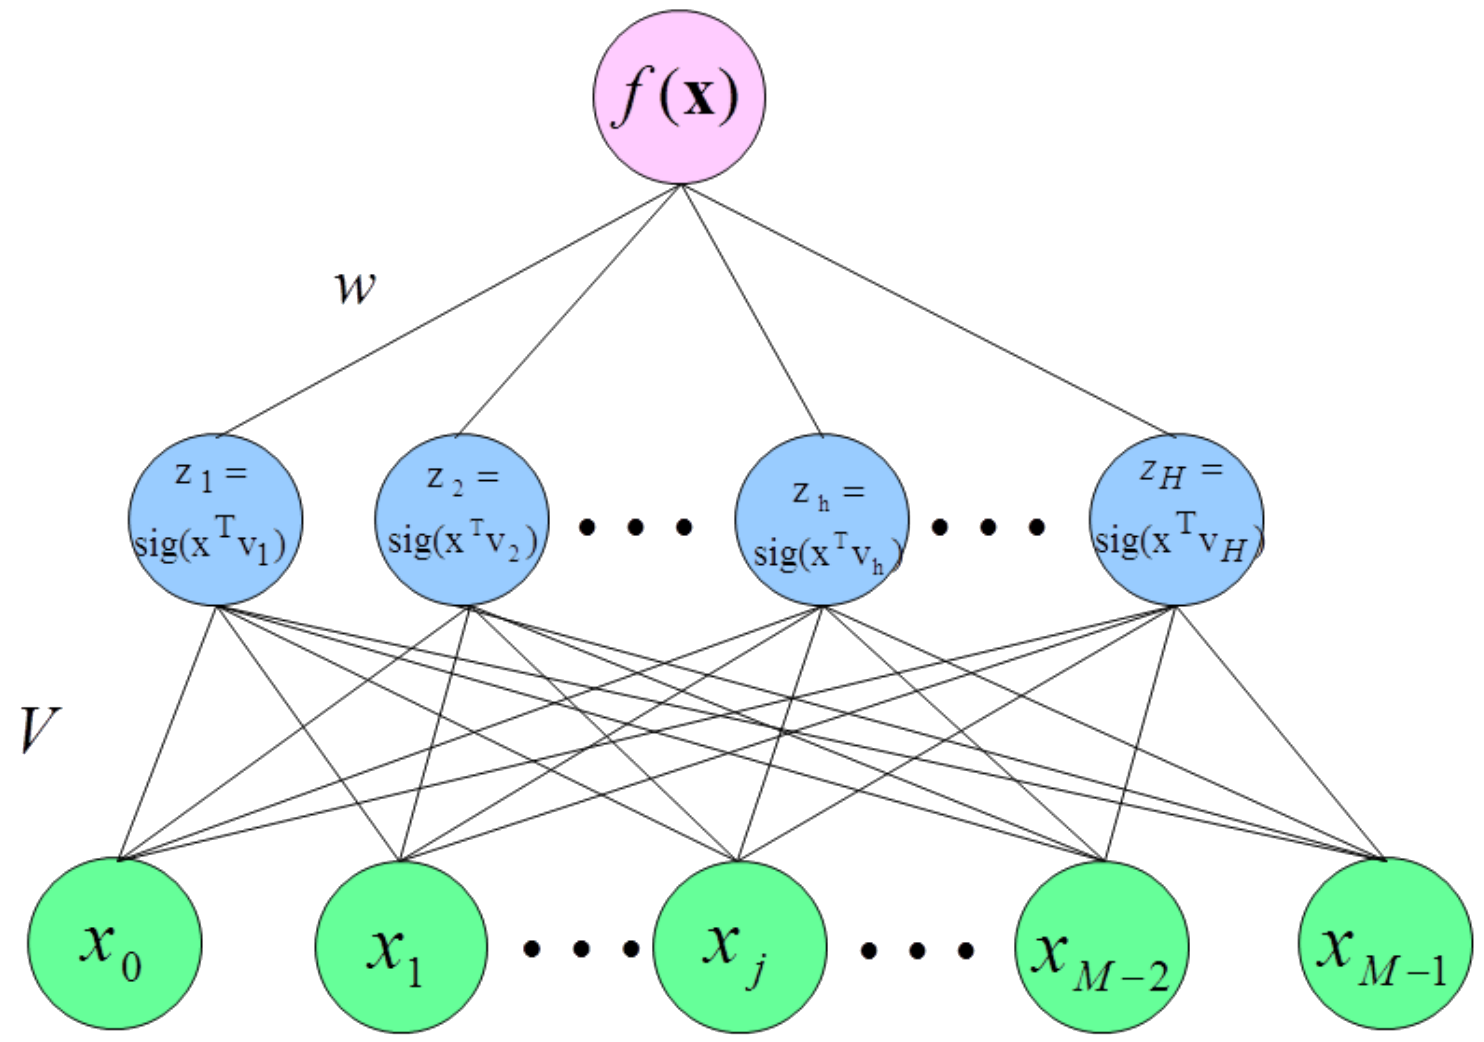
\includegraphics[width=\textwidth,height=0.4\textheight,keepaspectratio]{{{../res/Design of an artificial neural network}}}
	\caption{Design of an artificial neural network with one layer, $\pmb{x}$ as input, $z_i$ as activation function, $V$ und $w$ as weights and $f(\pmb{x})$ as prediction. Taken from~\cite{MachineLearning:NeuralNetworks}.}
	\label{fig:sample_neural_network_design}
\end{figure}

A rather simple feed-forward network is depicted in \autoref{fig:sample_neural_network_design}. Each line between two bubbles represents a connection, meaning the output of the bubble at the bottom is passed to the bubble at the top. The function used in calculating the various values for $z_i$ is called sigmoid (see~\cite{MachineLearning:NeuralNetworks}) and has an S-like shape. In terms of biology it can be though of as a boundary which has to be overcome prior to a signal being passed on. The references in the following paragraph are in regards to this figure.

Layers not representing the input or output are called hidden layers ({\color{blue}blue bubbles}). However the dimensions of an input ({\color{green}green bubbles}) are also referred to as features. The function of a node is called \textit{activation function} ($z_i$). The term \textit{learning} in the context of neural network refers to the process of adapting parameters or \textit{weights} ($V$ and $w$) of a nodes via a gradient which optimizes the desired function. The desired function is usually referred to as \textit{loss} and e.g. describes how many false classifications have been made. It is the job of the \textit{optimizer} to adapt the weights in a way which minimizes the function, a task usually done via propagating the error back through the network in a schema called \textit{back propagation}. The term \textit{training} refers to the process of applying the network to a set of data and adjusting the weights as necessary for each iteration. How many individual data points one of those iterations contains is described by the \textit{batch size}.

\chapter{Bayesian approach}
\label{chap:bayesian_approach}

\section{Simple Bayesian approach}
\label{sec:simple_bayes}

The goal of a Bayesian approach is to weight the particles' probability by their abundance in the sample. This process increases the likelihood of a particle being identified as belonging to a group with a higher abundance and decreases the likelihood of being identified as belonging to a group with a lower abundance. The approach depends on the detector yielding decay-agnostic results. Hence the detector shall be assumed to always output the likelihood of measuring the received signal given a specific particle hypothesis regardless of prior probabilities. Furthermore the approach assumes a bias towards one or a few particles in the sample since otherwise the a priori probabilities would be flat and therefore boil down to the same result.
Thankfully both of those hypothesis are given in the real world: The detector can be assumed to behaves independently of the relative particle abundance and the measured data usually shows a clear predominance of one or a few particle species.
This is not surprising in itself as the branching fractions are not equally distributed. Dictated by the laws of physics one particle species might be produced more frequently.

\begin{figure}[ht]
    \centering
    \includegraphics[width=\textwidth,height=0.4\textheight,keepaspectratio]{{{../res/charged 01/General Purpose Statistics: True Particle Abundances in the K+-Data}}}
    \caption{True particle abundance in the charged MC9 simulated data. \textit{NaN} stands for an invalid translation\protect\footnotemark from the particles' PDG code to an actual particle.}
    \label{fig:true_particle_abundance}
\end{figure}
\footnotetext{The error occurs due to the PDG code in the ROOT file being saved as \lstinline|float32| but some particle's code exceed the memory limit of $32$-bits. Notably, this effects the deuteron as well as its anti-particles.}

The absolute particle abundance of a sample taken from the Monte Carlo simulation of the charged decay of the $B$-mesons can be seen in \autoref{fig:true_particle_abundance}. In this example the bias towards pions and kaons can be clearly observed.

\begin{figure}[ht]
    \centering
    \includegraphics[width=\textwidth,height=0.4\textheight,keepaspectratio]{{{../res/charged 01/Diff Statistics: K Identification via PID, via flat Bayes}}}
    \caption{Comparisons of PPV and TPR for the Bayesian and standard PID approach for identifying kaons. The upper graph shows both rates of each approach separately using different colors, while the lower visualizes the ratio between the PPV's respectively the TPR's.}
    \label{fig:diff_stats_K_identification_via_pid_via_flat_bayes}
\end{figure}

\autoref{fig:diff_stats_K_identification_via_pid_via_flat_bayes} shows a comparison of the standard PID approach to the discussed Bayesian one. Using the Bayesian approach for identifying particles yields a very high positive predicted values even for low false positive rates as the introduced bias in the particle classification can utilize the unbalanced abundances. Furthermore the true positive rate of the Bayesian approach has a much steeper increase in comparison to the PID's one. However it levels of quicker, indicating that it fails to identify a few particles even at a high false positive rate.
The described effect can be seen for every stable particle with an ID and is not limited to the kaon. However it serves as a good example as it provides sufficient statistics for a throughout analysis.

\begin{figure}[ht]
    \centering
    \includegraphics[width=\textwidth,height=0.4\textheight,keepaspectratio]{{{../res/charged 01/Diff Heatmap: Heatmap of epsilonPID Matrix for an exclusive Cut via PID, via simple Bayes}}}
    \caption{Comparisons of the row-wised normed confusion matrix for the Bayesian and standard PID approach.}
    \label{fig:diff_heatmap_via_pid_via_flat_bayes}
\end{figure}

The improvements in the identification efficiencies are less obvious for an exclusive cut on the identifying variables. However in general the Bayesian approach is less prone to confusing particle with one another as seen in \autoref{fig:diff_heatmap_via_pid_via_flat_bayes}.

\section{Univariate Bayesian approach}
\label{sec:univariate_bayes}

The univariate Bayesian approach adds an dependency to one detector variable to the previous simple Bayesian approach. Hence instead of having a probability which depends on only on the particle abundance and the signal, the univariate approach additionally varies the probability depending on e.g. the transverse momentum. The most sensible variables are among others are said transverse momentum $p_t$ and the angle between the track of the particle and the beampipe $\Theta$.


\begin{appendix}
    %==================================================================
%\chapter{Anhang}
%==================================================================

%\label{sec-append}

%something
    \begin{thebibliography}{99}

\bibitem{pdg}
K. Nakamura et al. (Particle Data Group), JP G 37, 075021 (2010) and 2011 partial update for the 2012 edition (URL: http://pdg.lbl.gov)

\end{thebibliography}

\end{appendix}
\pagestyle{empty}
\cleardoublepage
\section*{Disclaimer}

\thispagestyle{empty}
\vspace*{0.8\textheight}
\noindent
I confirm that this \MakeLowercase{thesis} is my own work and I have documented all sources and material used.

\vspace{15mm}
\noindent
%\getSubmissionLocation{}, \getSubmissionDate{} \hspace{50mm} \getAuthor{}

\cleardoublepage{}

\cleardoublepage
\thispagestyle{empty}
\chapter*{Acknowledgments}

This thesis would not have been possible without the continues support of numerous people. First of all, I would like thank my supervisor Prof.~Dr.~Thomas~Kuhr for the chance to work in his research group as a Bachelor's student. By providing helpful and constructive feedback at every opportunity, he gave me inspiring insights into various topics of experimental particle physics. Of cource, I would also like to thank James~Kahn and Dr.~Martin~Ritter for providing profound answers to all of my questions.
Specifically, I would like to thank Dr.~Michael~Bender, Dr.~Martin~Ritter and Jakob~Roth as well for proofreading my thesis and giving valuable feedback.

Furthermore, thank you to all the students at the working group of Prof.~Dr.~Kuhr for their welcoming attitude and for making my stay an enjoyable time. Thank you, Christoph Ames, Anna Bertolini, Nan-Hee Kang, Yasin Silyanoglu, Daniel Moritz and Jakob Roth.

Last but not least, I would like to thank my family which has always supported me in countless ways.

Thank you all!


\end{document}


